% Copyright (c) 2014-2016 by the University of Waikato, Hamilton, NZ.
% This work is made available under the terms of the 
% Creative Commons Attribution-ShareAlike 3.0 license, 
% http://creativecommons.org/licenses/by-sa/3.0/. 
%
% Version: $Revision$

\documentclass[a4paper]{book}

\usepackage{wrapfig}
\usepackage{graphicx}
\usepackage{hyperref}
\usepackage{multirow}
\usepackage{scalefnt}
\usepackage{tikz}

% watermark -- for draft stage
\usepackage[firstpage]{draftwatermark}
\SetWatermarkLightness{0.9}
\SetWatermarkScale{5}

% Copyright (c) 2009 by the University of Waikato, Hamilton, NZ. 
% This work is made available under the terms of the 
% Creative Commons Attribution-ShareAlike 4.0 license,
% http://creativecommons.org/licenses/by-sa/4.0/.
%
% Version: $Revision: 5479 $

\newenvironment{tight_itemize}{
\begin{itemize}
  \setlength{\itemsep}{1pt}
  \setlength{\parskip}{0pt}
  \setlength{\parsep}{0pt}}{\end{itemize}
}

\newenvironment{tight_enumerate}{
\begin{enumerate}
  \setlength{\itemsep}{1pt}
  \setlength{\parskip}{0pt}
  \setlength{\parsep}{0pt}}{\end{enumerate}
}

% if you just need a simple heading
% Usage:
%   \heading{the text of the heading}
\newcommand{\heading}[1]{
  \vspace{0.3cm} \noindent \textbf{#1} \newline
}

\newcommand{\icon}[1]{\tikz[baseline=-3pt]\node[inner sep=0pt,outer sep=0pt]{\includegraphics[height=1.1em]{#1}};}


\title{
  \textbf{ADAMS} \\
  {\Large \textbf{A}dvanced \textbf{D}ata mining \textbf{A}nd \textbf{M}achine
  learning \textbf{S}ystem} \\
  {\Large Module: adams-meka} \\
  \vspace{1cm}
  
\includegraphics[width=2cm]{images/meka-module.png} \\
}
\author{
  Peter Reutemann
}

\setcounter{secnumdepth}{3}
\setcounter{tocdepth}{3}

\begin{document}

\begin{titlepage}
\maketitle

\thispagestyle{empty}
\center
\begin{table}[b]
	\begin{tabular}{c l l}
		\parbox[c][2cm]{2cm}{\copyright 2014-2016} &
		\parbox[c][2cm]{5cm}{
\includegraphics[width=5cm]{images/coat_of_arms.pdf}} \\
	\end{tabular}
	
\includegraphics[width=12cm]{images/cc.png} \\
\end{table}

\end{titlepage}

\tableofcontents
\listoffigures
%\listoftables

%%%%%%%%%%%%%%%%%%%%%%%%%%%%%%%%%%%
\chapter{Introduction}
The \textit{adams-meka} module integrates the MEKA \cite{meka} software suite 
in ADAMS.

\noindent From the MEKA homepage:
\begin{quote}
``The MEKA project provides an open source implementation of methods for 
multi-label classification and evaluation. It is based on the WEKA Machine 
Learning Toolkit. Several benchmark methods are also included, as well as the 
pruned sets and classifier chains methods, other methods from the scientific 
literature, and a wrapper to the MULAN framework.''
\end{quote}

%%%%%%%%%%%%%%%%%%%%%%%%%%%%%%%%%%%
\chapter{Flow}
The following source actors are available:
\begin{tight_itemize}
	\item \textit{MekaClassifierSetup} -- outputs a MEKA classifier setup.
\end{tight_itemize}
The following transformers are available:
\begin{tight_itemize}
	\item \textit{MekaClassifying} -- generates predictions on Instance objects
	using a trained model.
	\item \textit{MekaClassSelector} -- can turn any Instances object into
	a MEKA dataset by choosing which attributes to use as class attributes.
	\item \textit{MekaCrossValidationEvaluator} -- cross-validates a MEKA 
	classifier on the incoming dataset.
	\item \textit{MekaPrepareData} -- prepares Instances objects for the 
	use with MEKA classifiers.
	\item \textit{MekaResultSummary} -- turns the collected statistics from
	a MEKA evaluation run into a string.
	\item \textit{MekaResultValues} -- picks out selected statistics from a
	MEKA evaluation and generates a spreadsheet.
	\item \textit{MekaTrainClassifier} -- builds a MEKA classifier on the
	incoming dataset.
	\item \textit{MekaTrainTestSetEvaluator} -- evaluates a MEKA classifier
	on the incoming train/test split.
\end{tight_itemize}
The following sinks are available:
\begin{tight_itemize}
	\item \textit{MekaGraphVisualizer} -- displays graphs obtained from a model.
	\item \textit{MekaMacroCurve} -- displays macro-averaged curve.
	\item \textit{MekaMicroCurve} -- displays micro-averaged curve.
	\item \textit{MekaPrecisionRecall} -- displays precision-recall plots.
	\item \textit{MekaROC} -- displays ROC (receiver operator curve) plots.
\end{tight_itemize}

\newpage
Figures \ref{crossvalidate-flow} and \ref{crossvalidate-output} show a flow
and its associated output of cross-validating a MEKA classifier.

\begin{figure}[htb]
  \centering
  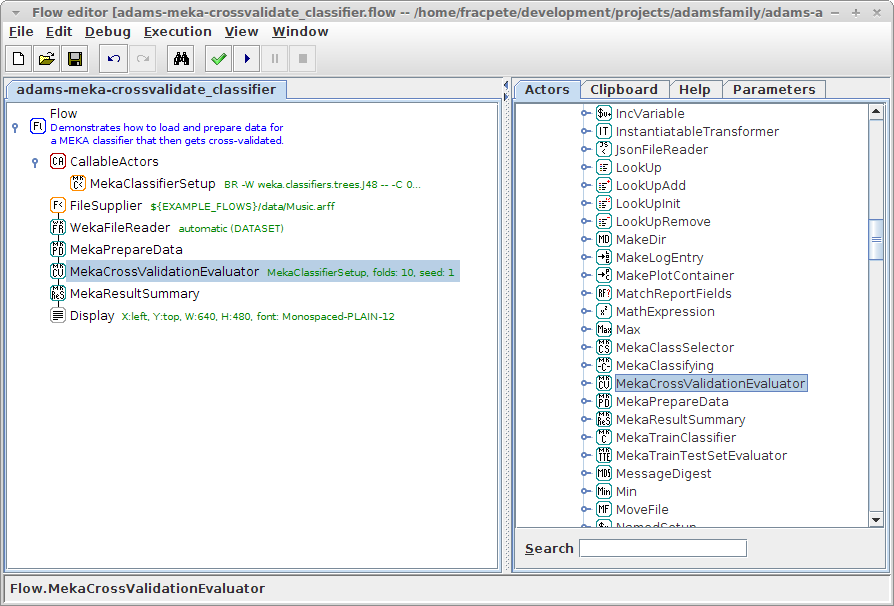
\includegraphics[width=12.0cm]{images/crossvalidate-flow.png}
  \caption{Flow for cross-validating a MEKA classifier.}
  \label{crossvalidate-flow}
\end{figure}

\begin{figure}[htb]
  \centering
  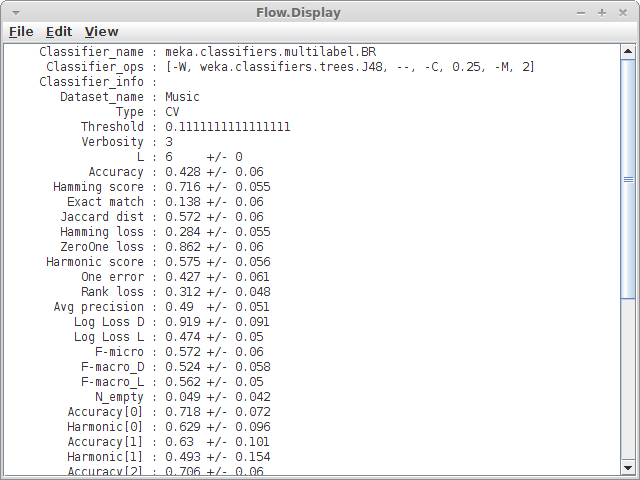
\includegraphics[width=8.0cm]{images/crossvalidate-output.png}
  \caption{The result of a cross-validated MEKA classifier.}
  \label{crossvalidate-output}
\end{figure}

%%%%%%%%%%%%%%%%%%%%%%%%%%%%%%%%%%%
\chapter{Tools}
The \textit{MEKA Explorer} can be launched from the main menu. It is located
in the \textit{Machine learning} section.

\begin{figure}[htb]
  \centering
  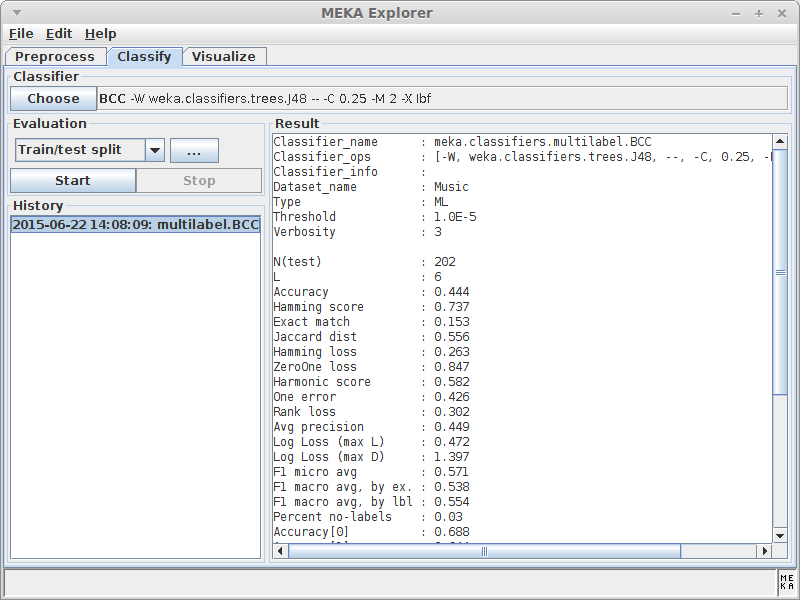
\includegraphics[width=12.0cm]{images/explorer.png}
  \caption{MEKA Explorer}
  \label{explorer}
\end{figure}


%%%%%%%%%%%%%%%%%%%%%%%%%%%%%%%%%%%
% Copyright (c) 2009-2012 by the University of Waikato, Hamilton, NZ. 
% This work is made available under the terms of the 
% Creative Commons Attribution-ShareAlike 4.0 license,
% http://creativecommons.org/licenses/by-sa/4.0/.
%
% Version: $Revision$

\begin{thebibliography}{999}
	% to make the bibliography appear in the TOC
	\addcontentsline{toc}{chapter}{Bibliography}

    % references
	\bibitem{adams}
		\textit{ADAMS} -- Advanced Data mining and Machine learning System \\
		\url{https://adams.cms.waikato.ac.nz/}{}
		
	\bibitem{heatmap}
		\textit{Heat map} -- WikiPedia article \\
		\url{http://en.wikipedia.org/wiki/Heat_map}{}

\end{thebibliography}


\end{document}
